\subsection{Index Construction}
\label{indexConstruction}
To build the CL-tree index, we propose two methods, {\tt basic} and {\tt advanced},
as presented in Section~\ref{basicIndex} and~\ref{advancedIndex}.

\subsubsection{The Basic Method}
\label{basicIndex}
As $k$-$\widehat {core}$s of a graph are nested naturally,
it is straightforward to build the CL-tree recursively in a top-down manner.
Specifically, we first generate the root node for $0$-core, which is exactly the entire graph.
Then, for each $k$-$\widehat {core}$ of $1$-core, we generate a child node for the root node.
After that, we only remain vertices with core numbers being $0$ in the root node.
Then for each child node, we can generate its child nodes in the similar way.
This procedure is executed recursively until all the nodes are well built.

\begin{algorithm}[h]
\caption{Index construction: {\tt basic}}
\label{alg:basicIndex}
\footnotesize{
\algrenewcommand{\algorithmiccomment}[1]{\hskip3em$//$ #1}
\begin{algorithmic}[1]
    \Function{buildIndex($G(V,E)$)}{}
        \State $core_G[\text{ }]\gets$ $k$-core decomposition on $G$;
        \State $k\gets$0, $root\gets (k, V)$;
        \State \Call{buildNode($root$, $0$)}{};
        \State build an inverted list for each tree node;
        \State \Return $root$;
    \EndFunction
    \Function{buildNode($root$, $k$)}{}
        \State $k\gets k+1$;
        \If{$k\leq k_{max}$}
            \State obtain $U_k$ from $root$;
            \State compute the connected components for the induced graph on $U_k$;
            %\luo{Do you mean "the connected components for the induced graph on $U_k$"?}
            \For {each connected component $C_i$}
                \State build a tree node $p_i\gets (k, C_i.vertexSet)$;
                \State add $p_i$ into $root.childList$;
                \State remove $C_i$'s vertex set from $root.vertexSet$;
                \State \Call{buildNode($p_i$, $k$)}{};
            \EndFor
        \EndIf
    \EndFunction
\end{algorithmic}}
\end{algorithm}


Algorithm~\ref{alg:basicIndex} illustrates the pseudocodes.
We first do $k$-core decomposition
using the linear algorithm~\cite{kcore2003},
and obtain an array $core_G[\text{ }]$(line 2),
where $core_G[i]$ denotes the core number of vertex $i$ in $G$.
We denote the maximal core number by $k_{max}$.
Then, we initialize the root node by the core number $k$=0 and $V$ (line 3).
Next, we call the function \textsc{buildNode} to build its child nodes (line 4).
Finally, we build an inverted list for each tree node and
obtain a well built CL-tree (lines 5-6).

In \textsc{buildNode}, we first update $k$ and obtain the vertex set $U_k$ from $root.vertexSet$,
which is a set of vertices with core numbers being at least $k$.
Then we find all the connected components from the subgraph induced by $U_k$ (lines 8-11).
Since each connected component $C_i$ corresponds to a $k$-$\widehat {core}$,
we build a tree node $p_i$ with core number $k$ and the vertex set of $C_i$,
and then link it as a child of $root$ (lines 12-14).
We also update $root$'s vertex set by removing vertices (line 15),
which are shared by $C_i$.
Finally, we call the \textsc{buildNode} function to build $p_i$'s child nodes recursively until all the tree nodes are created (line 16).

\textbf{Complexity analysis.}
The $k$-core decomposition can be done in $O(m)$.
The inverted lists of each node can be built in $O({\widehat l}\cdot n)$.
In function \textsc{buildNode}, we need to compute the connected components with a given vertex set,
which costs $O(m)$ in the worst case.
Since the recursive depth is $k_{max}$, the total time cost is $O(m\cdot {k_{\max }}+{\widehat l}\cdot n)$.
Similarly, the space complexity is $O(m+{\widehat l}\cdot n)$.

\subsubsection{The Advanced Method}
\label{advancedIndex}
While the {\tt basic} method is easy to implement,
it meets efficiency issues when both the given graph size and its $k_{max}$ value are large.
For instance, when given a clique graph with $n$ vertices (\textit{i.e.}, edges exist between every pair of nodes),
the value of $k_{max}$ is $n$--1. Therefore, the time complexity of the {\tt basic} method could be $O((m+{\widehat l})\cdot n)$,
which may lead to low efficiency for large-scale graphs.
To enable more efficient index construction, we propose the {\tt advanced} method,
whose time and space complexities are almost linear with the size of the input graph.

The {\tt advanced} method builds the CL-tree level by level in a bottom-up manner. Specifically, the tree nodes corresponding to larger core numbers are created prior to those with smaller core numbers. For ease of presentation, we divide the discussion into two main steps: creating tree nodes and creating tree edges.

\textbf{1. Creating tree nodes.} We observe that, if we acquire the vertices with core numbers at least $c$ and denote the induced subgraph on the vertices as $T_c$, then the connected components of $T_c$ have one-to-one correspondence to the $c$-$\widehat {core}$s. A simple algorithm would be, searching connected components for $T_c (0\leq c\leq k_{max})$ independently, followed by creating one node for each distinct component. This algorithm apparently costs $O(k_{max}\cdot m)$ time, as computing connected components takes linear time.
% given that the connected component search for a graph can be completed in linear time.

However, we can do better if we can incrementally update the connected components in a level by level manner (\textit{i.e.}, maintain the connected components of $T_{c+1}$ from those of $T_{c}$). We note that, such a node creation process is feasible by exploiting the classical \emph{union-find forest}~\cite{unionFind}. Generally speaking, the union-find forest enables efficient maintenance of connected components of a graph when edges are incrementally added. Using union-find forest to maintain connected components follows a process of edge examination. Initially, each vertex is regarded as a connected component. Then, edges are examined one by one. During the examine process, two components are merged together when encounters an edge connecting them. To achieve an efficient merge of components, the vertices in the component form a tree. The tree root acts as the representative vertex of the component. As such, merging two components is essentially linking two root vertices together. To guarantee the CL-tree nodes are formed in a bottom-up manner, we assign an examine priority to each edge. The priority is defined by the larger value of the two core numbers corresponding to the two end vertices of an edge. The edges associated to vertices with larger core numbers are examined first.

\textbf{2. Creating tree edges.} Tree edges are also inserted during the graph edge examination process.
In particular, when we examine a vertex $v$ with a set, $B$, of its neighbors, whose core numbers are larger than $core_G[v]$,
we require that the tree node containing $v$ should link to the tree node containing
the vertex, whose core number is the smallest among all the vertices in $B$.
Nevertheless, the classical union-find forest is not able to maintain such information. To address this issue, we thus propose an auxiliary data structure,
called \textbf{\underline{A}nchored \underline{U}nion-\underline{F}ind} (details of AUF are in Appendix~\ref{app:auf}),
based on the classical union-find forest.
We first define \emph{anchor vertex}.


\begin{definition}[Anchor vertex]
\label{def:anchor}
Given a connected subgraph $G'\subseteq G$,
the anchor vertex is the vertex with core number being $min\{core_G[v]|v\in G'\}$.
\end{definition}

The AUF is an extension of union-find forest, in which each tree has an anchor vertex,
and it is attached to the root node.
In CL-tree, for any node $p$ with corresponding $k$-$\widehat {core}$ ${\mathcal C}_k$,
its child nodes correspond to the $k$-$\widehat {core}$s,
which are contained by ${\mathcal C}_k$ and have core numbers being the most close to the core number of node $p$.
This implies that, when building the CL-tree in a bottom-up manner,
we can maintain the anchor vertices for the $k$-$\widehat {core}$s dynamically,
and they can be used to link nodes with their child nodes.
In addition, we maintain a vertex-node map,
where the key is a vertex and the value is the tree node contains this vertex,
for locating tree nodes.

\begin{algorithm}[h]
\caption{Index construction: {\tt advanced}}
\label{alg:advancedIndex}
\footnotesize{
\algrenewcommand{\algorithmiccomment}[1]{\hskip3em$//$ #1}
\begin{algorithmic}[1]
\Function{buildIndex($G(V,E)$)}{}
        \State $core_G[\text{ }]\gets$ $k$-core decomposition on $G$;
        \For {each $v\in V$}
            \Call{makeSet($v$)}{};
        \EndFor
        \State put vertices into sets $V_0, V_1, \cdots, V_{k_{max}}$;
        \State $k\gets k_{max}$, $map\gets \emptyset$;
        \While {$k\geq 0$}
            \State $V'\gets \emptyset$;
            \For {each $v\in V_k$}
                $V'$.add(\Call{find($v$)}{});
            \EndFor
            \State compute connected components for $V_{k}\cup V'$;
            \For {each component with vertex set $C_i$}
                \State create a node $p_i$ using ($k$, $\{C_i-V'\}$);
                \For {each $v \in \{C_i-V'\}$}
                    %\State $invertArr[v]\gets p_i$;
                    \State $map$.add($v$, $p_i$);
                    \For {each $ u \in v$'s neighbor vertices}
                        \If {$core_G[u]\geq core_G[v]$}
                            \State \Call{union($u$, $v$)}{};
                        \EndIf
                        \If {$core_G[u]>core_G[v]$}
                            \State $uRoot\gets$\Call{find($u$)}{};
                            \State $uAnchor\gets uRoot.anchor$;
                            %\State $p'\gets invertArr(uAnchor)$;
                            \State $p'\gets$ $map$.get($uAnchor$);
                            \State add $p'$ to $p$'s child List;
                        \EndIf
                    \EndFor
                    \State $vRoot\gets$\Call{find($v$)}{};
                    \If {$core_G[vRoot.anchor] > core_G[v]$}
                        \State \Call{updateAnchor($vRoot$, $core_G[\text{ }]$, $v$)}{};
                    \EndIf
                \EndFor
            \EndFor
            \State $k\gets k-1$;
        \EndWhile
        \State build the root node $root$;
        \State build an inverted list for each tree node;
        \State \Return $root$.
\EndFunction
\end{algorithmic}}
\end{algorithm}

Algorithm~\ref{alg:advancedIndex} presents the {\tt advanced} method.
Similar with {\tt basic} method, we first conduct $k$-decomposition (line 2).
Then, for each vertex, we initialize an AUF tree node (line 3).
We group all the vertices into sets (line 4),
where set $V_k$ contains vertices with core numbers being exactly $k$ (line 5).
Next, we initialize $k$ as $k_{max}$ and the vertex-node map $map$,
where the key is a vertex and the value is a CL-tree node whose vertex set contains this vertex.
In the while loop (lines 6-25),
we first find the set $V'$ of the representatives for vertices in $V_k$,
then compute the connected components for vertex set $V_k\cup V'$ (lines 7-9).
Next, we create a node $p_i$ for each component (lines 10-11).
For each vertex $v\in \{C_i-V'\}$, we add a pair ($v$, $p_i$) to the $map$ (lines 12-13).
Then for each of $v$'s neighbor, $u$, if its core number is at least $core_G[v]$,
we link $u$ and $v$ together in the AUF by a \textsc{union} operation (lines 14-16),
and find $p_i$'s child nodes using the anchor of the AUF tree (lines 17-21).
After vertex $v$ has been added into the CL-tree, we update the anchor (lines 22-24).
Then we move to the upper level in next loop (line 25).
After the while loop, we build the root node of the CL-tree (line 26).
Finally, we build the inverted list for each tree node and obtain the built index (lines 27-28).


\textbf{Complexity analysis.}
In Algorithm~\ref{alg:advancedIndex}, lines 1-3 can be completed in $O(m)$ (We assume $m$$\ge$$n$).
In the while loop, the number of operations on each vertex and its neighbors are constant,
and each can be done in $O(\alpha(n))$, where $\alpha(n)$, the inverse Ackermann function, is less than 5 for all remotely
practical values of $n$.
The keyword inverted lists of all the tree nodes can be computed in $O(n\cdot {\widehat l})$.
Therefore, the CL-tree can be built in $O(m\cdot \alpha(n)+n\cdot{\widehat l})$.
The space cost is $O(m+n\cdot{\widehat l})$, as maintaining an AUF takes $O(n)$.

%\textbf{Complexity analysis.}
%With our proposed AUF, we can reduce the complexity of CL-tree construction to $O(m\cdot \alpha(n))$,
%%which conforms to the complexity analysis of the classical union-find forest~\cite{unionFind}.
%where $\alpha(n)$, the inverse Ackermann function, is less than 5 for all remotely practical
%values of $n$~\cite{unionFind}.

\begin{example}
Figure~\ref{fig:advancedIndex} depicts an example graph with 14 vertices {$A,\cdots,N$}.
$V_i$ denotes the set of vertices whose core numbers are $i$.
When $k$=3, we first generate two leaf nodes $p_1$ and $p_2$,
then update the AUF, where roots' anchor vertices are in the round brackets.
When $k$=2, we first generate node $p_3$, then link it to $p_1$,
and then update the AUF forest.
When $k$=1, we first generate nodes $p_4$ and $p_5$.
Specifically, to find the child nodes of $p_4$,
we first find its neighbor $A$,
then find $A$'s parent $B$ using current AUF forest.
Since the anchor vertex of $B$ is $E$ and $E$ points to $p_3$ in the inverted array,
we add $p_3$ into $p_4$'s child List.
When $k$=0, we generate $p_6$ and finish the index construction.
\end{example}

\begin{figure}
	\small
	\centering
	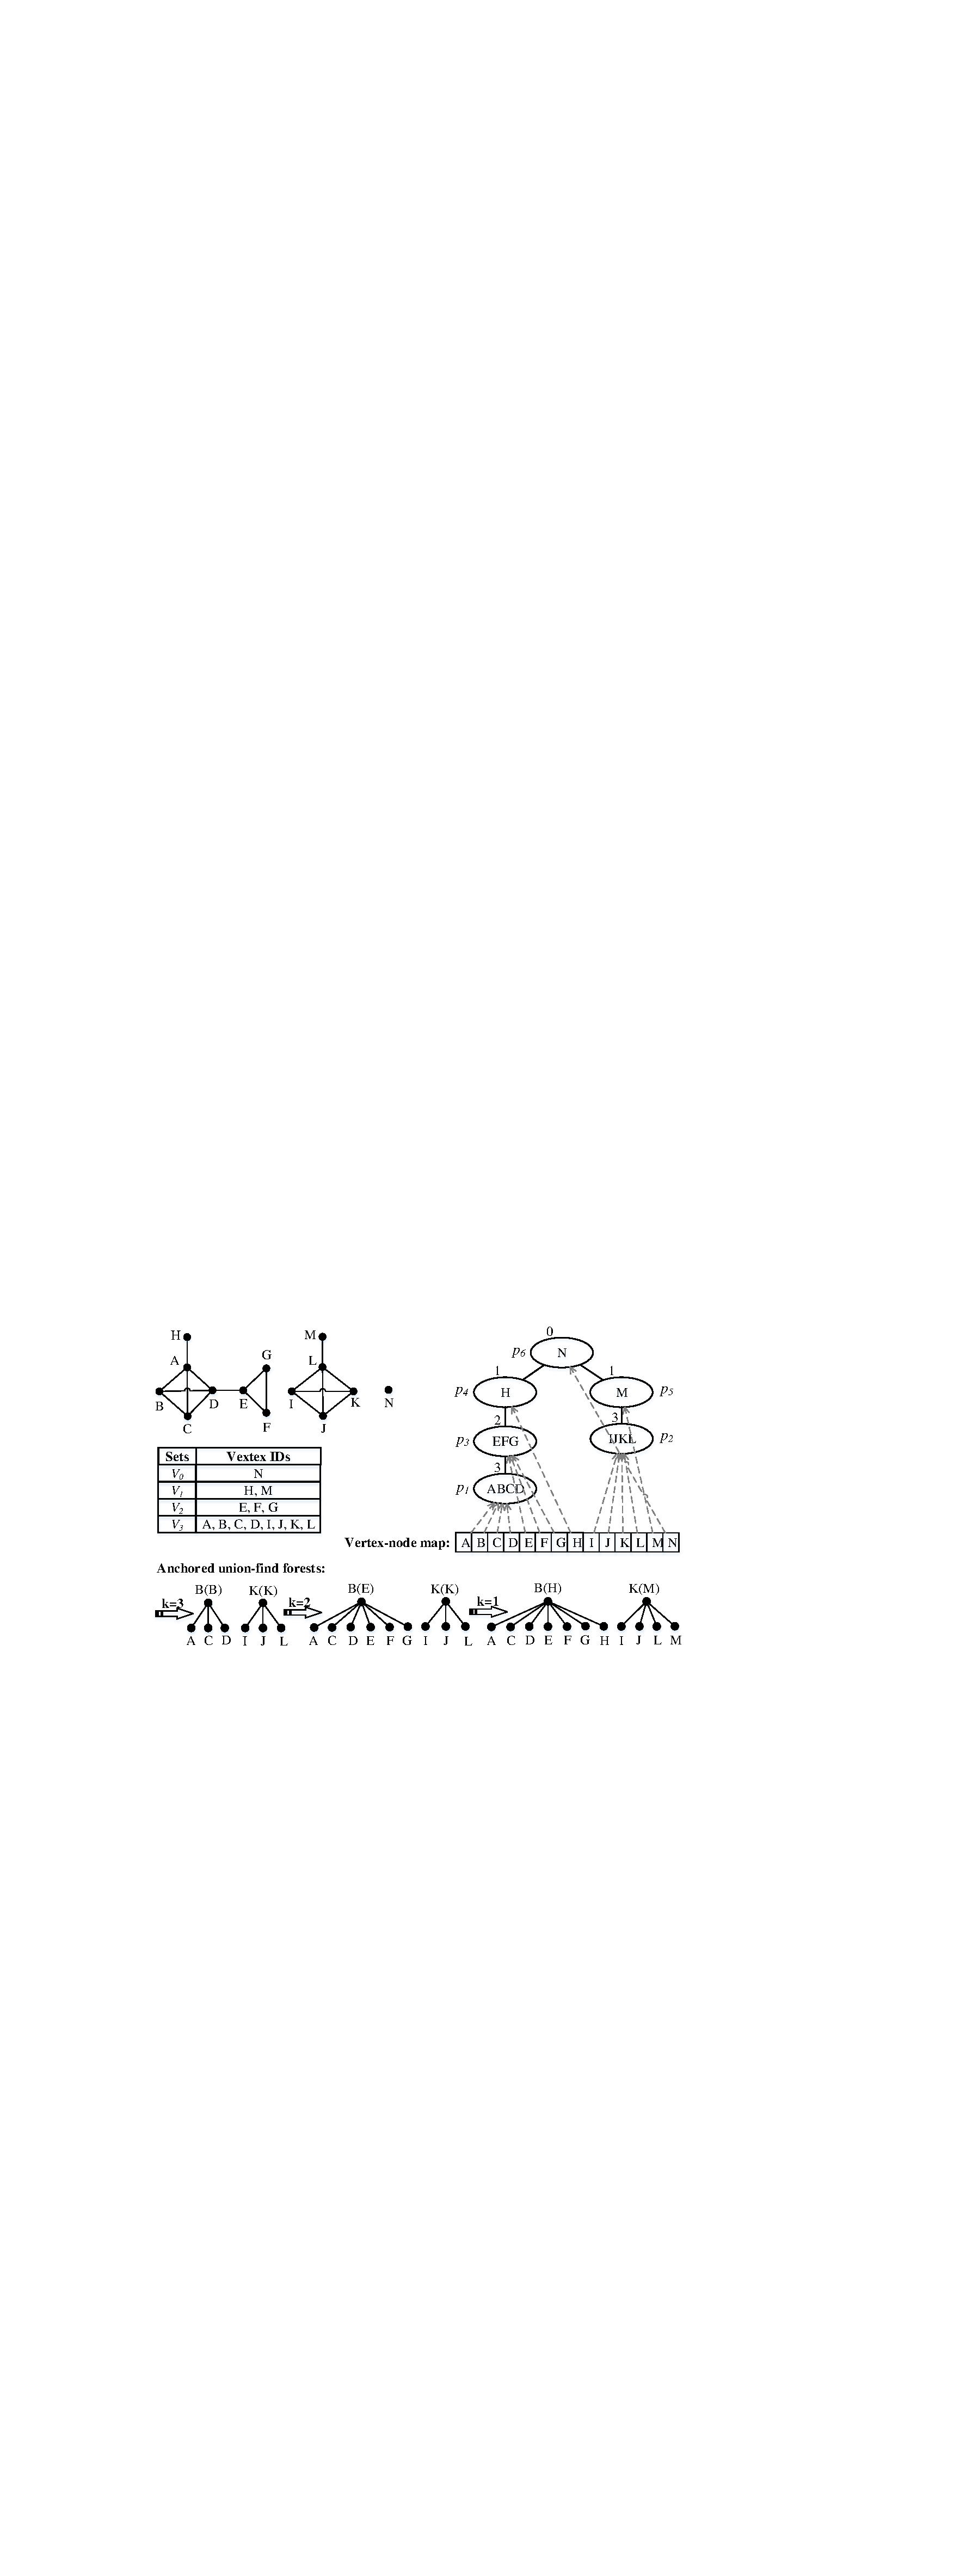
\includegraphics[width=0.88\linewidth]{figures/advancedIndex}
	\caption{An index built by {\tt advanced} method.}
	\label{fig:advancedIndex}
\end{figure} 